\hypersetup{linktocpage}

\hypersetup{colorlinks=false}
\setlength{\parskip}{0.5em}

\makeatletter
\renewcommand\theequation{S\@arabic\c@equation}
\makeatother

\renewcommand\Affilfont{\normalsize}

%%%%%%%%%%%%%%%%%%%%%%%%%%%%%%%%%%%%%%%%%%%%%%%%%%%%%%%
%%%%%%%%%%%%%%%%%%%%%%%%%%%%%%%%%%%%%%%%%%%%%%%%%%%%%%%
% \begin{document}

\renewcommand*\contentsname{\normalsize List of Supplementary Notes}
\makeatletter
\renewcommand{\tableofcontents}{\@starttoc{toc}}
\renewcommand*\l@section{\@dottedtocline{1}{0em}{6.3em}}
\let\l@table\l@content
\makeatother

\makeatletter
\renewcommand{\listoffigures}{\@starttoc{lof}}
\renewcommand*\l@figure{\@dottedtocline{1}{0em}{3.5em}}
\let\l@table\l@figure
\makeatother

\makeatletter
\renewcommand{\listoftables}{\@starttoc{lot}}
\renewcommand*\l@table{\@dottedtocline{1}{0em}{4.5em}}
\let\l@table\l@table
\makeatother

\renewcommand\thesection{Supplementary Note S\arabic{section}}
\makeatletter
\renewcommand*{\@seccntformat}[1]{\csname the#1\endcsname\hspace{0.5em}}
\makeatother

\renewcommand{\figurename}{\!\!}
\let\standardthefigure\thefigure
\renewcommand\thefigure{Figure S\standardthefigure}
% \addtolength{\cftfignumwidth}{15pt}

\renewcommand{\tablename}{\!\!}
\let\standardthetable\thetable
\renewcommand\thetable{Table S\standardthetable}

% \renewcommand{\algorithmname}{\!\!}
\let\standardthealgorithm\thealgorithm
\renewcommand\thealgorithm{S\standardthealgorithm}

\setcounter{figure}{0}

\section{Mapping function for $F$-MDS.} \label{sec:app1}

In this section, we explain a procedure of deriving a mapping function $f_\mathbf{z}(F_\mathbf{x})$ that is used to minimize an objective function for computing $F$-informed MDS.
The confirmatory term of the objective function (Equation 5 of the main text) is specifically designed to minimize a difference in $p$-values testing for group difference by representations under the original $S$- and two-dimensions. 
These \textit{p}-values are obtained from an empirical distribution of the pseudo-$F$s by permuted labels \cite{anderson01}. 
In other words, by denoting a label set as $[y_i]$ ($i=1,\cdots N$) and its permuted set as $[y_i^\pi]$ with operator $\pi$, we express each $F$-statistic as
\begin{equation}
\begin{aligned}
F^\pi_\mathbf{x} &= 
\left(\frac{\sum_{i,j}d_{ij}^2}{2\sum_{i,j}d_{ij}^2\,\1\{y_i^\pi = y_j^\pi\}} -1 \right) \cdot (N-2), \\
F^\pi_\mathbf{z} &= 
\left(\frac{\sum_{i,j}\|\mathbf{z}_i - \mathbf{z}_j\|_2^2}{2\sum_{i,j}\|\mathbf{z}_i - \mathbf{z}_j\|_2^2\,\1\{y_i^\pi = y_j^\pi\}} -1 \right) \cdot (N-2).
\label{eq:map1}
\end{aligned}
\end{equation}
% \end{align} 

It should be noted that the pseudo $F$-ratios can range differently based on how the samples are projected onto 2D. To scale between these two ratios and minimize the difference in $p$-values, we consider a mapping $f_\mathbf{z}: F_\mathbf{x} \rightarrow F_\mathbf{z}$ from a pair of ratios $(F_\mathbf{x}^{\pi_1}, F_\mathbf{z}^{\pi_2})$ where each element was ordered from two independent sets of repeated permutations. Figure below exemplifies how the $F$-ratios at each dimensionality scaled differently and depended on the choice of hyperparameter $\lambda$. In both settings, the $F$-ratio in $S$-dimension ranged between zero and six whereas in 2D representation the ratio ranged in [0,4]. The hyperparameter, however, impacted the detailed relationship between ordered $F_\mathbf{x}$ and ordered $F_\mathbf{x}$, when compared to each other. 

\begin{figure}[h]
    \centering
    \includegraphics[width=5.5in]{figures/supp-mds_Fval.pdf}
    \caption*{Figure: Mapping pseudo-$F$'s between two dimensionalities. Each $F_\mathbf{x} \text{-} F_\mathbf{z}$ relationship was obtained by permuting labels over 1,000 times, and by setting a hyperparameter $\lambda$ that is used to perform the majorization.}
    \label{fig:mds-fval}
\end{figure}

Using the mapping function $f_\mathbf{z}$, we now derive an exact form of confirmatory term proposed in the $F$-MDS objective function (Equation 5 of main text). The proposed form $\left|F_\mathbf{z} - f_\mathbf{z}(F_\mathbf{x})\right|$ measures how the 2D representation accurately reflected the $S$-dimensional distance structure with respect to the sample labels. Having the difference close to zero indicates that no additional update with the representation is required (let us denote it as $\mathbf{Z}^*$). Now by substituting the confirmatory term $\left|F_\mathbf{z} - f_\mathbf{z}(F_\mathbf{x})\right|$ with Equation \ref{eq:map1}, we define $\1\{y_i^\pi = y_j^\pi\}\coloneqq\epsilon_{ij}$ and write
\begin{align}
\mathbf{Z}^* &= \argmin_\mathbf{Z}\,\left|F_\mathbf{z} - f_\mathbf{z}(F_\mathbf{x})\right| \\
& = \argmin_\mathbf{Z}\,\left|(N-2)\cdot\left(\frac{\sum_{i,j}\|\mathbf{z}_i - \mathbf{z}_j\|_2^2}{2\sum_{i,j}\epsilon_{ij}\|\mathbf{z}_i - \mathbf{z}_j\|_2^2} -1 \right) - f_\mathbf{z}(F_\mathbf{x})\right| \\
&= \argmin_\mathbf{Z}\,\left|\frac{\sum_{i,j}\|\mathbf{z}_i - \mathbf{z}_j\|_2^2}{2\sum_{i,j}\epsilon_{ij}\|\mathbf{z}_i - \mathbf{z}_j\|_2^2} -1 - \frac{f_\mathbf{z}(F_\mathbf{x})}{N-2} \right| \\
&= \argmin_\mathbf{Z}\,\left| \frac{\sum_{i,j}\|\mathbf{z}_i - \mathbf{z}_j\|_2^2 - 2\sum_{i,j}\epsilon_{ij}\|\mathbf{z}_i - \mathbf{z}_j\|_2^2 \cdot [1+f_\mathbf{z}(F_\mathbf{x})/(N-2)]}{2\sum_{i,j}\epsilon_{ij}\|\mathbf{z}_i - \mathbf{z}_j\|_2^2} \right| \label{eq:pre_approx}\\
&\approx \argmin_\mathbf{Z}\,\left| \sum_{i,j}\|\mathbf{z}_i - \mathbf{z}_j\|_2^2 - 2\sum_{i,j}\epsilon_{ij}\|\mathbf{z}_i - \mathbf{z}_j\|_2^2 \cdot \left(1+\frac{f_\mathbf{z}(F_\mathbf{x})}{N-2}\right) \right| \label{eq:approx}\\
&= \argmin_\mathbf{Z}\,\left|\sum_{i,j} \left[1- 2\epsilon_{ij} \left(1+\frac{f_\mathbf{z}(F_\mathbf{x})}{N-2}\right)\right] \|\mathbf{z}_i - \mathbf{z}_j\|_2^2\right|,
\end{align}
where Equation \ref{eq:approx} is approximated from Equation \ref{eq:pre_approx} to ensure that the same physical dimension as the stress term was obtained. By substituting expression in Equation \ref{eq:pre_approx} with the proposed confirmatory term, we conclude by deriving the exact form of the $F$-MDS objective as
\begin{equation}
    O_{\rm FMDS}(\mathbf{Z}) = \sum_{i,j} (d_{ij} - \| \mathbf{z}_i - \mathbf{z}_j \|_2 )^2 + \lambda\left|\sum_{i,j} \left[1- 2\epsilon_{ij} \left(1+\frac{f_\mathbf{z}(F_\mathbf{x})}{N-2}\right)\right] \|\mathbf{z}_i - \mathbf{z}_j\|_2^2\right|.
\label{eq:fmds_objective}
\end{equation}

\clearpage



\section{Majorization algorithm.} \label{sec:app2}

We seek a configuration $\mathbf{Z^*}= (\mathbf{z}_1^*, \cdots \mathbf{z}_N^*)\in \bbr^{N\times 2}$ that minimizes an objective term for $F$-MDS, $O_{\text{FMDS}}(\mathbf{Z})$ (Equation \ref{eq:fmds_objective}).
Previous work by Witten \& Tibshirani \cite{witten11} suggests that MDS-based ordinations can be computed by applying the Majorization (or Majorize-Minimization) algorithm where to a quadratic expression in terms of $\mathbf{Z}$ is analytically solved. In detail, for every $k=1,\cdots N$, a point $\mathbf{z}_k^*$ minimizing $O_{\text{FMDS}}(\mathbf{Z})$, while other configuration points fixed, is written as
\begingroup
\allowdisplaybreaks
\begin{align}
\mathbf{z}_k^* 
&= \argmin_{\mathbf{z}_k}O_{\rm FMDS}(\mathbf{Z} | \mathbf{z}_1,\cdots \mathbf{z}_{k-1}, \mathbf{z}_{k+1}, \mathbf{z}_N) \\
&= \argmin_{\mathbf{z}_k}\, \sum_{i,j} (d_{ij} - \|\mathbf{z}_i - \mathbf{z}_j\|_2)^2 + \lambda\left|\sum_{i,j} \left[1- 2\epsilon_{ij} \left(1+\frac{f_\mathbf{z}(F)}{N-2}\right)\right] \|\mathbf{z}_i - \mathbf{z}_j\|_2^2\right| \\
&= \argmin_{\mathbf{z}_k}\, \sum_{j=1}^N (d_{jk} - \|\mathbf{z}_j - \mathbf{z}_k\|_2)^2 + \lambda\delta(\mathbf{z})\sum_{j=1}^N \left[1- 2\epsilon_{jk} \left(1+\frac{f_\mathbf{z}(F)}{N-2}\right)\right] \cdot \|\mathbf{z}_j - \mathbf{z}_k\|_2^2 \\
&= \argmin_{\mathbf{z}_k}\, \sum_{j=1}^N \left[1+\lambda\delta(\mathbf{z}) \left(1- 2\epsilon_{jk} \left(1+\frac{f_\mathbf{z}(F)}{N-2}\right)\right) \right] 
\|\mathbf{z}_k-\mathbf{z}_j\|_2^2 
- 2d_{jk}\|\mathbf{z}_k-\mathbf{z}_j\|_2
\label{eq:appc_mm1}
\end{align}
\endgroup
where we have defined $\delta (\mathbf{z})$ as
\begin{align}
\delta (\mathbf{z}) = \text{sign}\left\{\,\sum_{i,j} \left[1- 2\epsilon_{ij} \left(1+\frac{f_\mathbf{z}(F)}{N-2}\right)\right] \|\mathbf{z}_i - \mathbf{z}_j\|_2^2\right\}.
\end{align}

As described by \cite{borg97b}, applying the algorithm starts with majorizing with Equation \ref{eq:appc_mm1},
\begin{equation}
\sum_{j=1}^N\,
\left[1+\lambda\delta(\mathbf{z}) \left(1- 2\epsilon_{jk} \left(1+\frac{f_\mathbf{z}(F)}{N-2}\right)\right) \right] \|\mathbf{z}_k-\mathbf{z}_j\|_2^2 -
2d_{jk}\,\frac{\sum_{s=1}^2 (z_{ks}-z_{js})(\Tilde{z}_{ks}-z_{js})}{\|\Tilde{\mathbf{z}}_k-\mathbf{z}_j\|_2}, \label{eq:appc_mm2}
\end{equation}
where $\Tilde{\mathbf{z}}_k$ is a fixed term (not updated) while ${\mathbf{z}}_k$ still remains as a variable. We further assume that a change of mapping function $f_\mathbf{z}(F)$ is negligible and that $\delta(\mathbf{z})$ remains constant during the iteration (e.g., a small change in $\mathbf{z}_k$ from metric MDS). These allow us to approximate Equation \ref{eq:appc_mm2} with a quadratic expression in terms of $\mathbf{z}$ and proceed to its minimization analytically.
To find its minimum at $\mathbf{z}_{k}=\mathbf{z}_{k}^\dagger$, a derivative is taken with respect to $z_{ks}$ and is set to zero.
In other words, we obtain
\begin{align}
\begin{split}
0 = \sum_{j=1}^N\, \left[1+\lambda\delta(\mathbf{z}) \left(1- 2\epsilon_{jk} \left(1+\frac{f_\mathbf{z}(F)}{N-2}\right)\right) \right] (z_{ks}^\dagger - z_{js}) 
- d_{jk}\frac{\Tilde{z}_{ks}-z_{js}}{\|\Tilde{\mathbf{z}}_k-\mathbf{z}_j\|_2}.
\label{eq:mm_balance}
\end{split}
\end{align}

Noting that for a balanced design where $\sum_{j=1}^N \epsilon_{jk}= {N}/{2}$, for $k=1,\cdots N$, we rewrite Equation \ref{eq:mm_balance} and analytically obtain $z_{ks}^\dagger$:
\begin{align}
\begin{split}
& \sum_{j=1}^N\, \left[1+\lambda\delta(\mathbf{z}) \left(1- 2\epsilon_{jk} \left(1+\frac{f_\mathbf{z}(F)}{N-2}\right)\right) \right] z_{ks}^\dagger 
= \left( N - \frac{N\lambda\delta(\mathbf{z})f_\mathbf{z}(F)}{N-2} \right) z_{ks}^\dagger \\
&\qquad= \sum_{j=1}^N\, \left[1+\lambda\delta(\mathbf{z}) \left(1- 2\epsilon_{jk} \left(1+\frac{f_\mathbf{z}(F)}{N-2}\right)\right) \right] z_{js} + d_{jk}\frac{\Tilde{z}_{ks}-z_{js}}{\|\Tilde{\mathbf{z}}_k-\mathbf{z}_j\|_2}.
\end{split}
\end{align}
\begin{align}
\begin{split}
\therefore z_{ks}^\dagger = 
&\frac{(N-2)}{N(N-2) - N\lambda\delta(\mathbf{z}) f_\mathbf{z}(F)} \\
&\quad\times\left\{\sum_{j=1}^N\, \left[1+\lambda\delta(\mathbf{z}) \left(1- 2\epsilon_{jk} \left(1+\frac{f_\mathbf{z}(F)}{N-2}\right)\right) \right]  z_{js} + d_{jk}\frac{\Tilde{z}_{ks}-z_{js}}{\|\Tilde{\mathbf{z}}_k-\mathbf{z}_j\|_2}\right\}.
\label{eq:update_element}
\end{split}
\end{align}
Finally, rewriting Equation \ref{eq:update_element} in a vector form gives us an update rule of $\mathbf{Z}$ as below:
\begin{align}
\begin{split}
\mathbf{z}_k \gets
\frac{(N-2)}{N(N-2) - N\lambda\delta(\mathbf{z}) f_\mathbf{z}(F)}\cdot \left\{\sum_{j=1}^N\, \left[1+\lambda\delta(\mathbf{z}) \left(1- 2\epsilon_{jk} \left(1+\frac{f_\mathbf{z}(F)}{N-2}\right)\right) \right]  \mathbf{z}_{j} + d_{jk}\frac{\mathbf{z}_k -\mathbf{z}_j}{\|{\mathbf{z}}_k-\mathbf{z}_j\|_2}\right\}.
\label{eq:mm_update}
\end{split}
\end{align}

\clearpage



\section{Human gut microbiome dataset.} \label{sec:app3}

We retrieved two sets of human gut microbiome data from a publicly available repository \cite{Pasolli16}, previously generated from Shotgun Metagenomic Sequencing, where the reads were merged at the genus level \cite{reiman20}. 
The first dataset contained a gut microbiome derived from 118 healthy and 114 liver cirrhosis patients from a single study \cite{Qin14}.
The second includes samples from a human gut of 217 healthy and 223 patients with type 2 diabetes (T2D) from two separate studies \cite{Qin12, Karlsson13}.

For both datasets, a phylogenetic tree was generated using phyloT \cite{Letunic23} where branch lengths were uniformly assigned with unity, resulting in 268 (cirrhosis) and 216 (T2D) features or taxa respectively. Taxonomy and abundance table were obtained using the phylogenetic tree and the merged reads, respectively, which were then integrated via \texttt{phyloseq} (Bioconductor v3.18). Pairwise distance matrix $\mathbf{D}$ was computed based on the weighted Unifrac \cite{lozupone07}.

\clearpage



\section{Neural network model and architecture.} \label{sec:app4}

We sought to compare our $F$-MDS with neural network models that are used for dimensionality reduction. To convert compositional microbial abundance into a matrix with its phylogenetic information, we implemented PopPhy-CNN \cite{reiman20} architecture. Each converted matrix reflected a phylogenetic tree structure by bacterial 16S rRNA amplicon (amplicon sequence variant or ASV) and its relative abundance which is normalized by cumulative sum scaling (CSS) \cite{paulson13}.
Thirty-six bacterial community samples were retrieved and re-analyzed from the previous work \cite{kim22}. The samples represent balanced design of diatom-associated community with and without presence of the host. Each compositional sample was converted to a 2D array sized $10 \times 42$.
The data was randomly split into training and validation sets (6 and 30 each) using the stratified K-Fold.

\begin{figure}[ht]
    \centering
    \includegraphics[width=6in]{figures/supp-nn-eval.pdf}
    \caption*{Figure: Performance of self-supervised learning classifier by 50 training epochs. (A) Validation accuracy and (B) validation loss measured by categorical cross-entropy using bacterial community data represented as an image using PopPhy-CNN.}
    \label{fig:supp_nn_eval}
\end{figure}

The neural network architecture included an encoder consisting of one Gaussian noise filter, two 2D convolution layers (with kernel size of 5 by 3), and one fully connected layer with 32 output nodes. 
A self-supervised learning framework using SimCLR \cite{chen20} was chosen to explore its capability of arranging the microbiome data. The data augmentation was performed by applying random brightness and contrast filters with following parameters: (0.6, 0.2) for pretraining, (0.3, 0.1) for finetuning. In a pretraining step of SimCLR, a model was constructed by compiling encoder, projection head (two dense layers each of 32 output nodes), and one dense layer (10 output nodes). Site 1 and 2 datasets were individually trained and evaluated (30, 6 samples each) for the pretraining step, resulting a linear probing accuracy of 53.3\% after 50 training epochs (see Figure above). In the following finetuning step, the encoder is added with linear probe, resulting in a validation accuracy higher than 83.3\% after 50 epochs (see figure below). The trained encoder was used to obtain a 32 nodes-sized feature for each microbial community sample. The 32-dimensional feature was used for evaluating this neural network model with quality metrics.
Pairwise distance was calculated using $L_2$-squared metric to obtain Stress-1 and Shepard plot.

\clearpage



\section{Computational complexity.} \label{sec:app5}

We provide an upper bound of computational complexity of majorization algorithm for performing $F$-MDS.
Like most iteration-based optimizations, the computation cost of majorization was estimated on the basis of a single step.
We discuss the time complexity of each step outlined in Algorithms 1 and 2 of the main text.

For computing the mapping function (Algorithm 1), a pseudo-$F$-ratio is computed from a set of permuted labels $y^\pi$ and each of input matrices $d$, $\mathbf{z}$.
Each computation takes $\cO(N^2)$ operations with $N$ being the sample size.
The step repeats for a number of iteration, e.g., $p=999$, resulting in $\cO(2pN^2)$ operations.
Additional steps are taken to sort the lists of permuted $F$-ratios with $\cO(2N\log N)$.
In total, the complexity is $\cO(2pN^2 + 2N\log N)$.

For majorization step (Algorithm 2), the $F$-ratio is computed once and is mapped to $f_\mathbf{z}(F)$, taking $\cO(N^2 + \log N)$ operations.
Next, the sign of $F$-MDS confirmatory term $\delta(\mathbf{Z})$ is obtained and the step takes $\cO(N^2)$ operations.
Finally, the 2D representation $\mathbf{Z}$ is updated for every point, taking $\cO(N^2)$ operations.
Therefore, the complexity for one iteration of the majorization algorithm is $\cO(3N^2 + \log N)$.

In summary, the computational cost of performing $F$-MDS (unit iteration) is $\cO(2pN^2 + 3N^2 + 2N\log N + \log N) \approx \cO(pN^2)$. 
It is compared with other dimension reduction methods which is summarized below.

\begin{table}[h]
    \caption*{Comparison of time complexity between different dimensionality reduction methods.}
    \centering
    \begin{tabular}{c c c}
    \hline
       Method & Complexity & Algorithm \\
    \hline
        $F$-informed MDS\footnotemark & $\cO(pN^2)$ & Majorization \cite{borg97a} \\
        \multirow[c]{2}{*}{MDS} & $\cO(N^3)$ & Eigendecomposition \cite{Torgerson52} \\
         & $\cO(N\log N)$ & Divide-and-conquer \cite{Yang06} \\
        Supervised MDS$^1$ & $\cO(N^2)$ & Majorization \cite{witten11} \\
        UMAP & $\cO(N^{1.14})$ & NN-descent \cite{McInnes18, Dong11} \\
        \multirow{2}{*}{t-SNE$^1$} & $\cO(N^2)$ & Gradient descent \cite{maaten08} \\
         & $\cO(N\log N)$ & Barnes-Hut or dual-tree \cite{Maaten14} \\
        Isomap & $\cO(N^2\log N)$ & Dijkstra’s \cite{tenenbaum00, Pedregosa11} \\
    \hline
    \end{tabular}
    \label{tab:complexity}
\end{table}

\footnotetext[1]{Corresponds to a single iteration and does not represent a total complexity.}

\clearpage



\begin{figure}[h!]
    \centering
    \includegraphics[width=6.5in]{figures/Fig_S1.pdf}
    \caption[Pairs plot of simulated, binary dataset used in this study.]{Pairs plot of a simulated, binary dataset used in this study. Axes of each plot correspond to orthonormal vectors that were obtained through eigendecomposition of the design matrix $\mathbf{X}$. Alignment on the axis v1 indicates that the samples have been normalized (Equation 9, main text). Denoted with different colors and shapes are two groups that follow truncated normal distributions with different means but the same covariance (Equation 8, main text.) }
    \label{fig:sim_data_2d}
\end{figure}
\clearpage

\begin{figure}
    \centering
    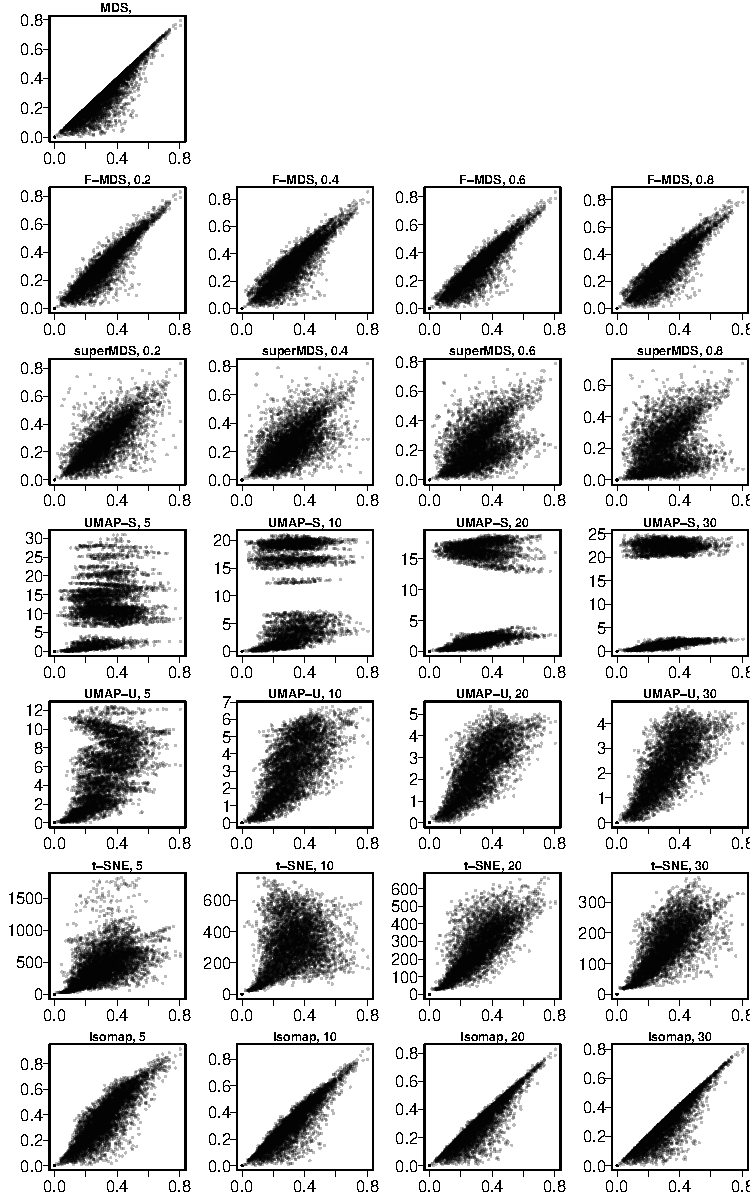
\includegraphics[width=5in]{figures/Fig_S2.pdf}
    \caption[Shepard plot from 4D simulated dataset with seven ordination methods.]{Shepard plot of simulated dataset (first replicate) using seven dimension reduction methods. The plots are titled with the respective method and hyperparameter values as follows: $\lambda$, $F$-MDS; $\alpha$, superMDS; Nearest neighbors number, supervised (-S) or unsupervised (-U) UMAP; Perplexity, t-SNE; Shortest dissimilarities number, Isomap. X- and Y-axis denote the pairwise distance in the original and embedding dimensions, respectively.}
    \label{fig:shepard_sim_all}
\end{figure}
\clearpage

\begin{figure}
    \centering
    \includegraphics[width=5in]{figures/Fig_S3.pdf}
    \caption[\textit{F}-correlation plot from simulated dataset.]{\textit{F}-correlation plot with simulated data. Pseudo $F$-ratios were calculated in the original dimension (x-axis) and in each dimension reduction method (y-axis) using first replicate of the simulated dataset. Pseudo $F$'s were calculated by randomly permuting labels by 500 times. Highlighted with red denotes the location of $F$'s from unpermuted labels. Each plot is titled with the method and hyperparameter used.}
    \label{fig:f_corr_sim_all}
\end{figure}
\clearpage

\begin{figure}
    \centering
    \includegraphics[width=5in]{figures/Fig_S4.pdf}
    \caption[Shepard plot from algal microbiome dataset with eight ordination methods.]{Shepard plot of algal-associated bacterial community data using eight dimension reduction methods. The plots are titled with the respective method and hyperparameter values as follows: $\lambda$, $F$-MDS; $\alpha$, superMDS; Nearest neighbors number, supervised (-S) or unsupervised (-U) UMAP; Perplexity, t-SNE; Shortest dissimilarities number, Isomap; none, neural network (NN). X- and Y-axis denote distances in the original and embedding dimensions, respectively.}
    \label{fig:shepard_alga_all}
\end{figure}
\clearpage

\begin{figure}
    \centering
    \includegraphics[width=5in]{figures/Fig_S5.pdf}
    \caption[\textit{F}-correlation plot from algal microbiome dataset.]{\textit{F}-correlation plot from algal microbiome dataset. Pseudo $F$-ratios comparing the original dimension (x-axis) and from eight dimension reduction methods (y-axis) with algal microbiome data. Pseudo $F$'s were calculated by randomly permuting labels by 500 times. Highlighted with red denotes the location of $F$'s from unpermuted labels. Each plot is titled with the method and hyperparameter used.}
    \label{fig:f_corr_alga_all}
\end{figure}
\clearpage

\begin{figure}
    \centering
    \includegraphics[width=6.5in]{figures/Fig_S6.pdf}
    \caption[Pairs plot of simulated, trinary data.]{Pairs plot of trinary, four-dimensional simulated data. Each row and column corresponds to respective axis for the projection. Denoted with different colors or shapes are the trinary groups that follow normal distributions with different means but the same covariance (Equation 10, main text.) }
    \label{fig:sim_data_4d}
\end{figure}
\clearpage

\begin{figure}
    \centering
    \includegraphics[width=6.5in]{figures/Fig_S7.pdf}
    \caption[Cluster centroid and variances of $F$-MDS representations.]{Cluster centroid and variances of $F$-MDS representations for simulated dataset (A-C) and algal microbiome (D-F). A,D: Distance between group centroids. B,E: Variance of each group measured in its long-axis. C,F: Variance of each group measured in its short-axis. For simulated dataset error bars denote standard deviation of triplicates. For variance calculations, blue and red colors denote group 1 and 2, respectively.}
    \label{fig:fmds_rep_analysis}
\end{figure}
\clearpage





% \end{document}